% This is "sig-alternate.tex" V2.1 April 2013
% This file should be compiled with V2.5 of "sig-alternate.cls" May 2012
%
% This example file demonstrates the use of the 'sig-alternate.cls'
% V2.5 LaTeX2e document class file. It is for those submitting
% articles to ACM Conference Proceedings WHO DO NOT WISH TO
% STRICTLY ADHERE TO THE SIGS (PUBS-BOARD-ENDORSED) STYLE.
% The 'sig-alternate.cls' file will produce a similar-looking,
% albeit, 'tighter' paper resulting in, invariably, fewer pages.
%
% ----------------------------------------------------------------------------------------------------------------
% This .tex file (and associated .cls V2.5) produces:
%       1) The Permission Statement
%       2) The Conference (location) Info information
%       3) The Copyright Line with ACM data
%       4) NO page numbers
%
% as against the acm_proc_article-sp.cls file which
% DOES NOT produce 1) thru' 3) above.
%
% Using 'sig-alternate.cls' you have control, however, from within
% the source .tex file, over both the CopyrightYear
% (defaulted to 200X) and the ACM Copyright Data
% (defaulted to X-XXXXX-XX-X/XX/XX).
% e.g.
% \CopyrightYear{2007} will cause 2007 to appear in the copyright line.
% \crdata{0-12345-67-8/90/12} will cause 0-12345-67-8/90/12 to appear in the copyright line.
%
% ---------------------------------------------------------------------------------------------------------------
% This .tex source is an example which *does* use
% the .bib file (from which the .bbl file % is produced).
% REMEMBER HOWEVER: After having produced the .bbl file,
% and prior to final submission, you *NEED* to 'insert'
% your .bbl file into your source .tex file so as to provide
% ONE 'self-contained' source file.
%
% ================= IF YOU HAVE QUESTIONS =======================
% Questions regarding the SIGS styles, SIGS policies and
% procedures, Conferences etc. should be sent to
% Adrienne Griscti (griscti@acm.org)
%
% Technical questions _only_ to
% Gerald Murray (murray@hq.acm.org)
% ===============================================================
%
% For tracking purposes - this is V2.0 - May 2012

\documentclass{sig-alternate-05-2015}

\usepackage{fancyvrb}

\begin{document}

% Copyright
\setcopyright{acmcopyright}
%\setcopyright{acmlicensed}
%\setcopyright{rightsretained}
%\setcopyright{usgov}
%\setcopyright{usgovmixed}
%\setcopyright{cagov}
%\setcopyright{cagovmixed}


% DOI
\doi{10.475/123_4}

% ISBN
\isbn{123-4567-24-567/08/06}

%Conference
\conferenceinfo{PLDI '13}{June 16--19, 2013, Seattle, WA, USA}

\acmPrice{\$15.00}

%
% --- Author Metadata here ---
\conferenceinfo{WOODSTOCK}{'97 El Paso, Texas USA}
%\CopyrightYear{2007} % Allows default copyright year (20XX) to be over-ridden - IF NEED BE.
%\crdata{0-12345-67-8/90/01}  % Allows default copyright data (0-89791-88-6/97/05) to be over-ridden - IF NEED BE.
% --- End of Author Metadata ---

\title{Is MFS Strongly Correlated with faulty code?
\titlenote{(Produces the permission block, and
copyright information). For use with
SIG-ALTERNATE.CLS. Supported by ACM.}}
%\subtitle{
%\titlenote{A full version of this paper is available as
%\textit{Author's Guide to Preparing ACM SIG Proceedings Using
%\LaTeX$2_\epsilon$\ and BibTeX} at
%\texttt{www.acm.org/eaddress.htm}}}
%
% You need the command \numberofauthors to handle the 'placement
% and alignment' of the authors beneath the title.
%
% For aesthetic reasons, we recommend 'three authors at a time'
% i.e. three 'name/affiliation blocks' be placed beneath the title.
%
% NOTE: You are NOT restricted in how many 'rows' of
% "name/affiliations" may appear. We just ask that you restrict
% the number of 'columns' to three.
%
% Because of the available 'opening page real-estate'
% we ask you to refrain from putting more than six authors
% (two rows with three columns) beneath the article title.
% More than six makes the first-page appear very cluttered indeed.
%
% Use the \alignauthor commands to handle the names
% and affiliations for an 'aesthetic maximum' of six authors.
% Add names, affiliations, addresses for
% the seventh etc. author(s) as the argument for the
% \additionalauthors command.
% These 'additional authors' will be output/set for you
% without further effort on your part as the last section in
% the body of your article BEFORE References or any Appendices.

\numberofauthors{5} %  in this sample file, there are a *total*
% of EIGHT authors. SIX appear on the 'first-page' (for formatting
% reasons) and the remaining two appear in the \additionalauthors section.
%
\author{
% You can go ahead and credit any number of authors here,
% e.g. one 'row of three' or two rows (consisting of one row of three
% and a second row of one, two or three).
%
% The command \alignauthor (no curly braces needed) should
% precede each author name, affiliation/snail-mail address and
% e-mail address. Additionally, tag each line of
% affiliation/address with \affaddr, and tag the
% e-mail address with \email.
%
% 1st. author
\alignauthor
Xintao Niu\\
       \affaddr{State Key Laboratory for Novel Software Technology}\\
       \affaddr{Nanjing University}\\
       \affaddr{China, 210023}\\
       \email{niuxintao@gmail.com}
% 2nd. author
\alignauthor
Changhai Nie\\
       \affaddr{State Key Laboratory for Novel Software Technology}\\
       \affaddr{Nanjing University}\\
       \affaddr{China, 210023}\\
       \email{changhainie@nju.edu.cn}
% 3rd. author
\alignauthor
Xiaoyin Wang \\
       \affaddr{Department of Computer}\\
       \affaddr{Science}\\
       \affaddr{The University of }\\
       \affaddr{Texas at San Antonio}\\
 %      \affaddr{China, 211171}\\
%       \email{xujiaxi@njxzc.edu.cn} \\
       \email{Xiaoyin.Wang@utsa.edu}
 % use '\and' if you need 'another row' of author names
 \and
% 4th. author
\alignauthor
Hareton Leung \\
       \affaddr{Department of computing}\\
       \affaddr{Hong Kong Polytechnic University}\\
       \affaddr{Kowloon, Hong Kong}\\
       \email{hareton.leung@polyu.edu.hk}
\alignauthor
Jeff Lei \\
       \affaddr{Department of Computer}\\
       \affaddr{Science and Engineering }\\
       \affaddr{The University of Texas at Arlington}\\
%       \affaddr{Arlington, Texas}\\
       \email{ylei@cse.uta.edu}
%% 6th. author
%\alignauthor Charles Palmer\\
%       \affaddr{Palmer Research Laboratories}\\
%       \affaddr{8600 Datapoint Drive}\\
%       \affaddr{San Antonio, Texas 78229}\\
%       \email{cpalmer@prl.com}
}
% There's nothing stopping you putting the seventh, eighth, etc.
% author on the opening page (as the 'third row') but we ask,
% for aesthetic reasons that you place these 'additional authors'
% in the \additional authors block, viz.
%\additionalauthors{Additional authors: John Smith (The Th{\o}rv{\"a}ld Group,
%email: {\texttt{jsmith@affiliation.org}}) and Julius P.~Kumquat
%(The Kumquat Consortium, email: {\texttt{jpkumquat@consortium.net}}).}
%\date{30 July 1999}
% Just remember to make sure that the TOTAL number of authors
% is the number that will appear on the first page PLUS the
% number that will appear in the \additionalauthors section.

\maketitle
\begin{abstract}
Combinatorial Testing (CT) is an effective technique for testing the interactions of factors in the Software Under Test(SUT). Most works in CT focus on the method itself, e.g., how to generate test cases, model the inputs, or handle the constraints of the inputs. Few of the works consider the justification of CT, i.e., is detecting and identifying the failure-inducing interactions really useful and helpful to code-level fault diagnosis? In this paper, we novelty studied the relationship between the failure-inducing interactions and code which causes the failure. Specifically, based on symbolic execution, we firstly obtain the guaranteed code of the corresponding failure-inducing interactions, i.e., those program entities which are directly affected by these interactions. And then we will compared these guaranteed code with those real faulty code to see whether there exists any associations between failure-inducing interactions with these real faulty code. Our empirical studies based on 5 real subjects showed that the failure-inducing interactions are strongly correlated with faulty code in the SUT.

\end{abstract}


%
% The code below should be generated by the tool at
% http://dl.acm.org/ccs.cfm
% Please copy and paste the code instead of the example below.
%

\begin{CCSXML}
<ccs2012>
<concept>
<concept_id>10011102.10011103</concept_id>
<concept_desc>Software defect analysis~Software testing and debugging</concept_desc>
<concept_significance>500</concept_significance>
</concept>
</ccs2012>
\end{CCSXML}

\ccsdesc[500]{Software defect analysis~Software testing and debugging}
%\ccsdesc{Reliability Verification~a}
%\ccsdesc[100]{Networks~Network reliability}

%
%\category{D.2.5}{Software Engineering}{Testing and debugging}[Debugging aids,testing tools]
%
%\terms{Reliability, Verification}


%
% End generated code
%

%
%  Use this command to print the description
%
\printccsdesc

% We no longer use \terms command
%\terms{Theory}

\keywords{Software Testing, Combinatorial Testing, Symbolic execution, Failure-inducing interactions, Guaranteed code}


\section{Introduction}
Modern software is becoming more and more complex. To test such software is challenging, as the candidate factors that can influence the system's behaviour, e.g., configuration options, system inputs, message events, are enormous. Even worse, the interactions between these factors can also crash the system, e.g., the incompatibility problems. In consideration of the scale of the industrial software, to test all the possible interactions of all the factors (we call them the interaction space) is not feasible, and even if it is possible, it is not wise to test all the interactions because most of them do not provide any useful information.
%Further more, it is a standard . airline

Many empirical studies show that, in real software systems, the effective interaction space, i.e., targeting fault detection, makes up only a small proportion of the overall interaction space \cite{kuhn2002investigation,kuhn2004software}. What's more, the number of factors involved in these effective interactions is relatively small, of which 4 to 6 is usually the upper bounds\cite{kuhn2002investigation}. With this observation, applying Combinatorial testing(CT) in practice is appealing, as it is proven to be effective to detect the interaction faults in the system.

CT tests software with a elaborate test suite which checks all the required parameter value combinations, and after detecting some failures by this test suite, it then identify the failure-inducing interactions, or more formally, failure-causing schemas (MFS) in the SUT. Most works in CT focus on the method itself, e.g, to design smaller test suite with the same interaction coverage \cite{cohen1997aetg,cohen2003augmenting,lei2008ipog,jia2015learning}, or to identify the MFS more accurately \cite{martinez2009locating,nie2011minimal,zhang2011characterizing,niu2013identifying}. Few of the works consider the following question:

\emph{Is detecting and identifying the MFS really useful and helpful to code-level fault diagnosis?}

To analyse this question is important and necessary, because it will build the relationship between MFS and faulty code, which is the foundation to apply CT on code-level debugging. In this paper, we try to answer this question by studying the \emph{guaranteed code} of interactions. The \emph{guaranteed code} of a interaction is the program entities (e.g., statements, branches, blocks, etc.) which are directly \emph{affected} by the interaction according to the previous study \cite{reisner2010using}. Obtaining the guaranteed code of an interaction can help us understand how this interaction influence on the behaviour of the program under test. Furthermore, analysing the guaranteed code of the MFS can offer us an insight into the extent to which the MFS is related to the cause of the failure; based on which, we can learn whether detecting and identifying the MFS can facilitate the debugging, as well as bug fixing.

%To compute the MFS of the SUT,
%
%With respect to the guaranteed code.
%
%To compute the guaranteed code of the interaction, We need to utilize symbolic execution. Specifically, we accumulated added on symbolic, and find those guaranteed code. We define the .

%
There are many techniques to compute the MFS in CT. In this paper, we adopts our previous method proposed in \cite{nie2011minimal}, which is one of the most common MFS identification technique in CT. With respect to guaranteed code, we follow the steps which are original proposed in \cite{reisner2010using}, which firstly utilizes symbolic execution tool to search possible paths for different values assigned to the input parameters, and then calculates the guaranteed code for each possible interaction based on these paths. One difference from study in \cite{reisner2010using} is that we only need to compute the guaranteed code for the MFS we identified in the SUT, instead of all the possible interactions. After obtaining the MFS and corresponding guaranteed codes, we will evaluate the correlation between MFS and faulty code.

We have design several empirical studies on 5 open-source software subjects. These studies considers several different aspects (e.g., the degree of MFS, the types of faults) of the relationships between MFS and faulty code. Our results suggests that: 1) The MFS does relate to the faulty code to some extent; 2) For different types of faults, the correlation between MFS and faulty code varies;  3) The input model of the program under test significantly impacts on this correlation.

%These faults include injected and real ones. We first model their input and computed the MFS and also the guaranteed code of these MFS. We observe their relationships between these code with those real faulty statement. One observation in our case study shows that .  Besides this, we also compare . The results shows that .

%\textbf{Contributions:}

The remaindering of this paper are organised as follows: Section \ref{sec:pre} gives the preliminaries about Combinatorial testing (especially MFS-related), and basic definitions about Guaranteed code. Section \ref{sec:research} proposes three research questions that needs to be handled in this paper. Section \ref{sec:subjects} introduces the subjects on which our experiments are conducted on. Section \ref{sec:results} shows the results as well as the analysis. Section \ref{sec:related} discusses the related works.  Section \ref{sec:conclusion} concludes this paper.

\section{Preliminary}\label{sec:pre}
This section presents some formal definitions about MFS and guaranteed code.

\subsection{Basic definitions about CT}\label{sec:pre:ct}

Assume that the Software Under Test (SUT) is influenced by \emph{n} parameters, and each parameter $p_{i}$ can take the values from the finite set $V_{i}$, $|V_{i}|$ = $a_{i}$ ($i$ = 1,2,..n). We will give some basic definitions which are related to failure-inducing interactions in CT.

\newdef{definition}{Definition}
\begin{definition}
A \emph{test case} of the SUT is a tuple of \emph{n} values, one for each parameter of the SUT. It is denoted as  ($v_{1}$, $v_{2}$,...,$v_{n}$), where $v_{1}\in V_{1}$, $v_{2} \in V_{2}$ ... $v_{n} \in V_{n}$.
\end{definition}
%a \emph{n}-tuple

In practice, these parameters in the test case can represent many factors, such as input variables, run-time options, building options or various combination of them. We need to execute the SUT with these test cases to ensure the correctness of the behaviour of the SUT.

%\begin{definition}
%We consider any abnormally executing test case as a \emph{fault}. It can be a thrown exception, compilation error, assertion failure or constraint violation. When faults are triggered by some test cases, it is desired to figure out which parameter values in these test cases are the failure-inducing ones.
%Some subsets of these test cases should be analysed.
%\end{definition}


\begin{definition}
For the SUT, the \emph{n}-tuple (-,$v_{x_{1}}$,...,$v_{x_{k}}$,...)is called a \emph{k}-degree \emph{schema} ($0 < k \leq n $) when some k parameters have fixed values and other irrelevant parameters are represented as "-".
\end{definition}

For example, the tuple (-, 4, 4, -) is a 2-degree schema. In effect a test case itself is a k-degree \emph{schema}, when k = n. Furthermore, if a test case contains a \emph{schema}, i.e., every fixed value in the schema is in this test case, we say this test case \emph{contains} the \emph{schema}.
%, which can be denoted as $k-value\  combination \in T$

Note that the schema is a formal description of the interaction between parameter values we discussed before.

\begin{definition}
Let $c_{l}$ be a \emph{l}-degree schema, $c_{m}$ be an \emph{m}-degree schema in SUT and $l < m$. If all the fixed parameter values in $c_{l}$ are also in $c_{m}$, then $c_{m}$ \emph{subsumes} $c_{l}$. In this case we can also say that $c_{l}$ is a \emph{sub-schema} of $c_{m}$ and $c_{m}$ is a \emph{super-schema} of $c_{l}$, which can be denoted as $c_{l} \prec  c_{m}$.
\end{definition}

For example,  the 2-degree schema (-, 4, 4, -) is a sub-schema of the 3-degree schema (-, 4, 4, 5), that is, (-, 4, 4, -) $\prec$ (-, 4, 4, 5).

\begin{definition}
If all test cases that contain a schema, say $c$, trigger a particular fault, say $F$, then we call this schema $c$ the \emph{faulty schema} for $F$. Additionally, if none of sub-schema of $c$ is the \emph{faulty schema} for $F$, we then call the schema $c$ the \emph{minimal failure-causing schema (MFS)} \cite{nie2011minimal} for $F$.

%Based on this, if a test case $t$ hit such a failure-inducing combination, say $c(F)$, it should trigger the fault $F$, for which the test case can be put as $t(F)$
\end{definition}

Note that MFS is identical to the failure-inducing interaction discussed previously. In this paper, the terms \emph{failure-inducing interactions} and \emph{MFS} are used interchangeably.
%Figuring the MFS out helps to identify the root cause of a failure and thus facilitate the debugging process.

\subsection{Identification of MFS}\label{sec:pre:mfs}
When a test case fails during test case, we are still far from figuring out the MFS \cite{colbourn2008locating,martinez2008algorithms,martinez2009locating}, as we do not know exactly which schemas in the failed test cases should be responsible for the failure. For example, if test case (0, 0, 0, 0) failed during testing, there are six 2-degree candidate failure-inducing schemas, which are (0, 0, -, -), (0, -, 0, -), (0, -, -, 0) , (-, 0, 0, -), (-, 0, -, 0), (-, -, 0, 0), respectively. Without
additional information, it is difficult to figure out the specific schemas in this suspicious set that caused the failure. Considering that the failure can be triggered by schemas with other degrees, e.g., (0, -, -, -) or (0, 0, 0, -), the problem of MFS identification becomes more complicated.

In fact, for a failing test case ($v_{1},v_{2},...,v_{n}$), there can be at most $2^{n} - 1$ possible schemas for the MFS. Hence, more test cases should be generated to identify the MFS. Next, we will show how MFS identification processes with an example.

Consider an program like Fig \ref{toy-program}, which contains four integer parameters: a, b, c, and d. With respect to applying combinatorial testing, we need to first build a input model for this program. For simplicity, let a, b, c and d can take on the following values:  $v_{a} = \{ 1, 2\}$, $v_{b} = \{ 0, 1\}$, $v_{c} = \{ 1, 2\}$, and $v_{d} = \{ 0, 1\}$, respectively. Assume that through testing of this program, we find a test case, e.g., (a = 1, b = 0, c = 1, d = 1), will trigger an arithmetic exception. Then we will describe how CT identify the MFS in this test case.

%taking square root of a negative number
\begin{figure}
\begin{Verbatim}[numbers=left,xleftmargin=5mm]
public float foo(int a, int b, int c, int d){
  int x, y, z;
  x = 4;
  if(a < 2){
    y = 3;
    if(c < 2){
            z =  Math.sqrt(y - x);
            return z / y;
    }
    else
        return x + y;
  }
  else{
    y = 2;
    if(b < 1){
        if(d < 1)
            return y / (x + y);
        else
            return x / (x + y);
    }
    else
        return y * x;
  }
}
\end{Verbatim}
\caption{A simple program \emph{foo} with four input parameters}
\label{toy-program}
\end{figure}

A typical MFS identification process is shown in Table \ref{ofot-identify}. In this table, test case $t$ represents the failing test case we aforementioned. To identify the MFS, we mutate one factor of \emph{t} one time to generate new test cases: $t_{1}$ -- $t_{4}$.  It turns out that test case $t_{1}$ passed, which indicates that this test case break the MFS in the original test case \emph{t}. So (1, -, -, -) should be a failure-causing factor. Similarly, we can also conclude that (-, -, 1, -) is another failure-inducing factor because of the pass of $t_{3}$. Considering that all the other test cases failed, which means no other failure-inducing factors were broken, therefore, the MFS in \emph{t} is (1, -, 1, -).

\begin{table}[ht]
\caption{OFOT example}
\label{ofot-identify}
\center
\begin{tabular}{llllll}
 \hline
\multicolumn{5}{c}{\bfseries Original test case} & \bfseries Outcome \\  \hline
 $t$ & \multicolumn{4}{l}{1 \ \ \ \ 0 \ \ \ \  1 \ \ \ \ 1 } & Fail \\
 \hline
\multicolumn{5}{c}{\bfseries Additional  test cases} &  \\  \hline
$t_{1}$ &\multicolumn{4}{l}{2  \ \ \ \  0 \ \ \ \  1 \ \ \ \ 1 }& Pass \\
$t_{2}$ &\multicolumn{4}{l}{1  \ \ \ \  1 \ \ \ \  1 \ \ \ \ 1 } & Fail \\
$t_{3}$ &\multicolumn{4}{l}{1  \ \ \ \  0 \ \ \ \  2 \ \ \ \ 1 } & Pass \\
$t_{4}$ &\multicolumn{4}{l}{1  \ \ \ \  0 \ \ \ \  1 \ \ \ \ 0 } & Fail \\
 \hline
\end{tabular}
\end{table}

This identification process mutate one factor of the original test case at a time to generate extra test cases. Then according to the outcome of the test cases execution result, it will identify the MFS of the original failing test cases. It is called the OFOT method \cite{nie2011minimal}, which is a well-known MFS identification method in CT. In this paper, we will focus on this identification method.
%It should be noted that the following proposed CT framework can be easily applied to other MFS identification methods.


\subsection{Basic definitions about guaranteed code}\label{sec:pre:guar}
Although MFS are the failure-inducing parts of the failing test input for the SUT, however, we still cannot directly utilize it for fault localization, because they do not provide any code-level information. For this, we need to build the relationship between input schemas and program entities.

Let $\mathcal{P}$ be a path in the SUT. Then let $Cov(\mathcal{P})$ = $< s_{1}, s_{2}, s_{3},... s_{n} >$ be the program entities that covered by path $\mathcal{P}$. A program entity can be a statement, block, edges, etc. In this paper, we mainly focus on statements; note that other types of structure coverage can also be applied \cite{song2012itree}. Let $Pcon(\mathcal{P})$ = $<pc_{1}, pc_{2}, pc_{3}, ... pc_{k}>$ be the path conditions that are encountered by path $\mathcal{P}$.  As an example, consider the program list in Fig \ref{toy-program}. It is easy to find that it has five possible paths, which forms the execution tree in Fig \ref{foo-tree}.

\begin{figure}
 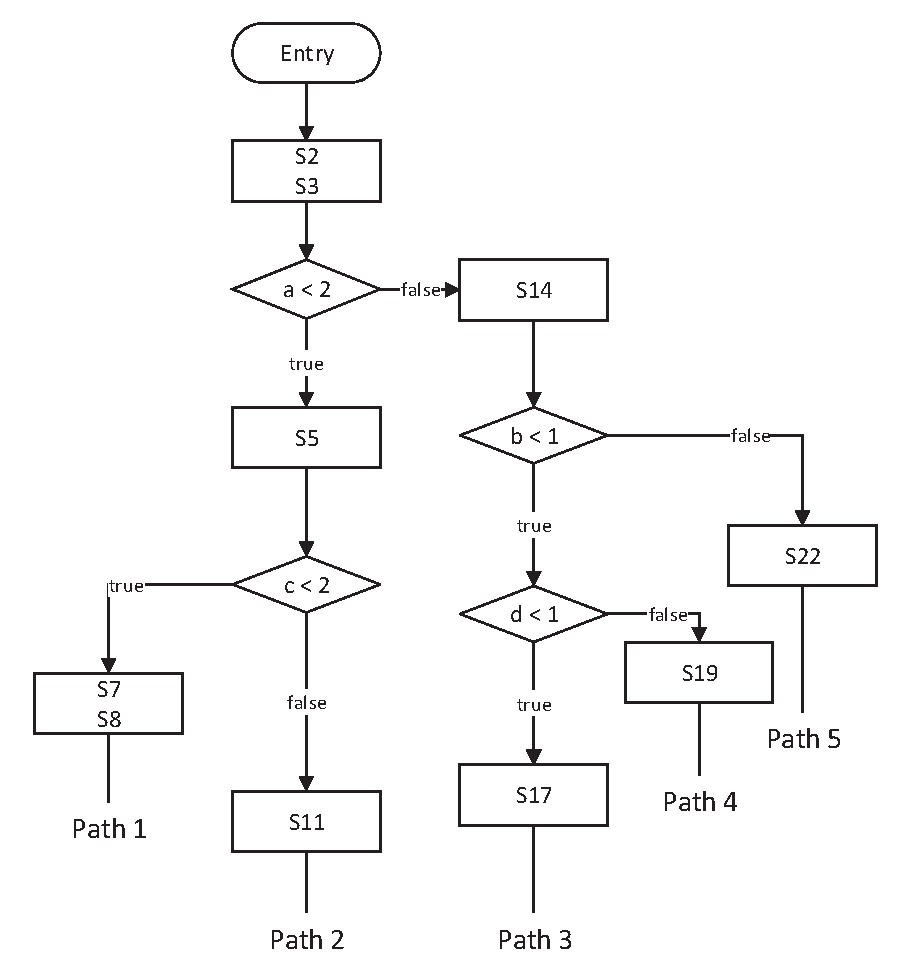
\includegraphics[width=3.4in]{foo_tree.eps}
\caption{The execution tree of program \emph{foo}}
\label{foo-tree}
\end{figure}

In this tree, a rhombus node represents a path condition, and a rectangle represents the statement. Note that those consecutive statements are included in one rectangle. From this figure, we can list the paths, their covered entities, and their path conditions, which are explicitly shown in Table \ref{cov-con-foo}.

\begin{table}[ht]
\caption{Paths, covered entities, and conditions of \emph{foo}}
\label{cov-con-foo}
\center
\begin{tabular}{lll}
 \hline
\bfseries ID & \bfseries Covered Entities & \bfseries Path Conditions \\  \hline
 $1$ & S2, S3, S5, S7, S8& $a < 2$,  $c < 2$\\
 $2$ & S2, S3, S5, S11 & $a < 2$,  $\neg c < 2$\\
 $3$ & S2, S3, S14, S17& $\neg a < 2$,  $b < 1$, $d < 1$\\
 $4$ & S2, S3, S14, S19& $\neg a < 2$,  $b < 1$, $\neg d < 1$\\
 $5$ & S2, S3, S14, S22& $\neg a < 2$,  $\neg b < 1$\\
 \hline
\end{tabular}
\end{table}


Next we will give some important definitions that are related to the guaranteed code.
%For simplicity, we next use notation $c^\sharp$ indicates a logic expression meaning that the parameter values are equal to those in schema $c$.

\begin{definition}
For a schema $c$, and a path $\mathcal{P}$, if all the path conditions in this path can be satisfied when given an input that contains this schema, we call $\mathcal{P}$ the \emph{Consistent path} of schema $c$, which can be denoted as $SAT(Pcon(\mathcal{P}) \bigwedge c)$.
\end{definition}

In fact, to judge whether a path is the \emph{consistent path} of one schema, is to find whether exist an input that contains this schema and follows all the path conditions of this path. Taking the program \emph{foo} for example, Path 1 is the consistent path of schema (1, -, -, -), because $( a < 2 $ $\wedge $ $c < 2 $ $\wedge $ $a = 1 )$  $= true $ can be solved, e.g., input (1, 1, 1, 1) is such a result.

Based on this definition, we use the notation $c^{\sharp}$ to represent the set of all the consistent paths of schema $c$. Then we will give the formal definition of weak guaranteed of one schema.

\begin{definition}
For a schema $c$, the weak guaranteed code of $c$, i.e., $wg(c)$, is the intersection of program entities covered by its consistent paths. Formally, $wg(c)$ = $\bigcap_{\mathcal{P} \in c^{\sharp}} Cov(\mathcal{P})$.

\end{definition}

As an example, we list some schemas, and their corresponding consistent paths and weak guaranteed code in Table \ref{weg-foo}.


\begin{table}[ht]
\caption{weak guaranteed code of some schemas of \emph{foo}}
\label{weg-foo}
\center
\begin{tabular}{lll}
 \hline
\bfseries Schema & \bfseries $c^{\sharp}$ & \bfseries $wg(c^{\sharp})$\\  \hline
 $(1, -, -, -)$ & S2, S3, S5, S7, S8& $a < 2$,  $c < 2$\\
 $(1, -, 1, -)$ & S2, S3, S5, S11 & $a < 2$,  $\neg c < 2$\\
 $(2, 1, -, -)$ & S2, S3, S14, S17& $\neg a < 2$,  $b < 1$, $d < 1$\\
 $(2, 1, -, 1)$ & S2, S3, S14, S19& $\neg a < 2$,  $b < 1$, $\neg d < 1$\\
 $(2, 1, 1, 1)$ & S2, S3, S14, S22& $\neg a < 2$,  $\neg b < 1$\\
 \hline
\end{tabular}
\end{table}

Essentially, the weak guaranteed code\footnote{The definition of weak guaranteed code is similar to the \emph{guarantee coverage} defined in \cite{reisner2010using}. The difference is that in this paper we do not distinguish the input and value symbolic; instead, they are handled in an unified way.} of one schema, is the maximal common code that is expected to be executed by any path which consists with this schema. In other word, this schema guarantees some code to be executed.

%\footnote{Weak guaranteed is ,
%Strong guaranteed is Note that this is the same to the interactions in paper. To let different, we }.

%Note that the definitions is one different from original defined, . which we do not consider input, instead, they are also modeled as symbolic. Based on This, all the input can be handled unified as the same way as those symbolic values.



Although the weak guaranteed code always follows with the corresponding schema, it does not necessarily indicates that the schema directly controls the weak guaranteed code. This is because there may exists some other schemas that control some part of this weak guaranteed code, but these schemas may always appears with the corresponding schema. Obviously, these schemas are the sub-schemas of this schema. For example, in Fig, .

Hence, to understand which code are under the direct control of some schemas, we need to remove the influence from their subschemas.
%Considering this, it may in fact the behaviour under the sub-schema . For example, in Fig.  Hence, to totally reflect the influence behaviour of sub-schemas, we need to remove the impact from the sub-schemas.

\begin{definition}
For a schema $c$, the strong guaranteed code of $c$, i.e., $sg(c)$, is the weak guaranteed code of $c$ with removing those weak guaranteed code of its subschemas. Formally, $sg(c)$ = $wg(c) \backslash \{\bigcup_{c' \prec c} wg(c') \}$.

\end{definition}

Strong guaranteed code are the program entities that under the direct control of the corresponding schema, and hence it reflects how the schema influence on the behaviour of program. As an example, .


In this paper, we focus on the guaranteed code of MFS, instead of all the other schemas in the test case. With respect to this example, it is easily find that the weak guaranteed code and strong guaranteed code is,  respectively. They are very correlated to the real faulty code, especially for the strong guaranteed code, .  However, in the real situation, it may . As we want to know whether to detect and identify the MFS is really helpful in the code-based diagnosis, we need to do more empirical studies to find the result.


%\subsection{The method to get guaranteed code}\label{sec:pre:getguar}
%
%We need to first utilize the symbolic executions.
%
%Then for the MFS we need to compute the consisient, we need a smt solver to solve this problem.
%definition guaranteed code
%
%definition minimal guaranteed code
%%

%
%In this paper, we use the symbolic execution to . The details is as follwos:




%\section{A case study}
%This section will provide an example to show how to



\section{Research questions} \label{sec:research}
To comprehensive study the correlativeness between the MFS and real


\subsection{The correlation between MFS and faulty code}


Hence, it motivates our first research question:

\textbf{Q1: Is MFS correlated to the faulty code?}

This question is key to. We let the guaranteed code of MFS.


\subsection{The influence of different types of faults}


Q2: Different fault type?

Taks as an example.

\subsection{The influence of inputs model}

Q3: Is the building model affected  MFS ?

Taks as an example.


These questions are important, as

\section{Subject programs}\label{sec:subjects}

\subsection{Generating faulty programs}

\subsection{Symbolic execution of the paths}


%\section{Getting MFS and their guaranteed code}

\section{Results}\label{sec:results}



\subsection{Threats to Validation}


\section{Related works}\label{sec:related}

There are many methods aims at identifying MFS in CT, which can be classified into two categories:



1. MFS in CT


All these methods. with respect to the code level which utilizes.
2. use MFS to isolate faulty code. machunhyan \cite{ma2013locating}  and leiyu \cite{ghandehari2013fault}


Studies on symbolic execution, has .

4. Use symoblic execution in CT. Charles song \cite{reisner2010using} first. Then extend to itree \cite{song2012itree}, then extends to multiple leaves with \cite{song2014itree}.

Our work differs from them

\section{Conclusions and Future works}\label{sec:conclusion}

%\end{document}  % This is where a 'short' article might terminate

%ACKNOWLEDGMENTS are optional
%\section{Acknowledgments}

%
% The following two commands are all you need in the
% initial runs of your .tex file to
% produce the bibliography for the citations in your paper.
\bibliographystyle{abbrv}
\bibliography{sigproc}  % sigproc.bib is the name of the Bibliography in this case
% You must have a proper ".bib" file
%  and remember to run:
% latex bibtex latex latex
% to resolve all references
%
% ACM needs 'a single self-contained file'!
%
%APPENDICES are optional
%\balancecolumns
\appendix
%Appendix A
%\section{Headings in Appendices}
%The rules about hierarchical headings discussed above for
%the body of the article are different in the appendices.
%In the \textbf{appendix} environment, the command
%\textbf{section} is used to
%indicate the start of each Appendix, with alphabetic order
%designation (i.e. the first is A, the second B, etc.) and
%a title (if you include one).  So, if you need
%hierarchical structure
%\textit{within} an Appendix, start with \textbf{subsection} as the
%highest level. Here is an outline of the body of this
%document in Appendix-appropriate form:
%\subsection{Introduction}
%\subsection{The Body of the Paper}
%\subsubsection{Type Changes and  Special Characters}
%\subsubsection{Math Equations}
%\paragraph{Inline (In-text) Equations}
%\paragraph{Display Equations}
%\subsubsection{Citations}
%\subsubsection{Tables}
%\subsubsection{Figures}
%\subsubsection{Theorem-like Constructs}
%\subsubsection*{A Caveat for the \TeX\ Expert}
%\subsection{Conclusions}
%\subsection{Acknowledgments}
%\subsection{Additional Authors}
%This section is inserted by \LaTeX; you do not insert it.
%You just add the names and information in the
%\texttt{{\char'134}additionalauthors} command at the start
%of the document.
%\subsection{References}
%Generated by bibtex from your ~.bib file.  Run latex,
%then bibtex, then latex twice (to resolve references)
%to create the ~.bbl file.  Insert that ~.bbl file into
%the .tex source file and comment out
%the command \texttt{{\char'134}thebibliography}.
%% This next section command marks the start of
%% Appendix B, and does not continue the present hierarchy
%\section{More Help for the Hardy}
%The sig-alternate.cls file itself is chock-full of succinct
%and helpful comments.  If you consider yourself a moderately
%experienced to expert user of \LaTeX, you may find reading
%it useful but please remember not to change it.
%\balancecolumns % GM June 2007
% That's all folks!
\end{document}
